% ********** Rozdział 2 **********
\chapter{Opis struktury projektu}

{Projekt ten został zrealizowany z wykorzystaniem nowoczesnych technologii programistycznych. Głównym językiem programowania jest C\#, znany ze swojej wszechstronności i wydajności, co czyni go idealnym wyborem dla aplikacji multimedialnych. Aplikacja korzysta z frameworka Entity Framework do zarządzania bazą danych, co pozwala na efektywne i bezproblemowe przechowywanie oraz dostęp do danych użytkownika. Interfejs użytkownika został zbudowany z wykorzystaniem Avalonia, nowoczesnego frameworka GUI, który zapewnia płynne i atrakcyjne wizualnie doświadczenie użytkownika.}

\section{Kluczowe Technologie i Narzędzia w Projekcie}

\begin{itemize}
    \item \textbf{ .NET 6:}  Jako kompleksowe środowisko uruchomieniowe i framework programistyczny, .NET 6 oferuje wydajność, bezpieczeństwo i wsparcie dla wielu platform, co jest niezbędne dla nowoczesnych aplikacji. Umożliwia ono tworzenie wydajnej i skalowalnej aplikacji, zapewniając jednocześnie wsparcie dla najnowszych standardów i praktyk programistycznych.
    \item \textbf{ Avalonia :} Jest frameworkiem do tworzenia interfejsów użytkownika, który umożliwia tworzenie aplikacji działających na wielu platformach. W projekcie "Music Player", Avalonia jest wykorzystywana do stworzenia atrakcyjnego i responsywnego interfejsu użytkownika, który jest spójny na różnych systemach operacyjnych. Dzięki swojej elastyczności i wsparciu dla XAML, Avalonia idealnie nadaje się do budowy nowoczesnych aplikacji multimedialnych, takich jak "Music Player", oferując zaawansowane funkcje GUI, takie jak animacje, style i szablony.
    
    \item \textbf{ Repozytorium kodu Github:}  Jest to platforma do hostingu kodu źródłowego, która wykorzystuje system kontroli wersji Git. Umożliwia przechowywanie, zarządzanie i śledzenie zmian w kodzie projektów. 
    \item \textbf{ GitHub Actions:} Jest to narzędzie CI/CD (Continuous Integration/Continuous Deployment) zintegrowane z GitHubem, które umożliwia automatyzację różnych etapów rozwoju oprogramowania, takich jak testowanie, budowanie i wdrażanie aplikacji. W projekcie "Music Player", GitHub Actions jest używany do automatycznego budowania projektu, co jest widoczne w pliku dotnet-build.yml. Ten plik definiuje zadania, które są wykonywane automatycznie przy każdym pushu lub pull requeście, zapewniając ciągłą integrację i sprawdzanie jakości kodu.
    \item \textbf{ Baza Danych MySQL:} Jest to popularny system zarządzania relacyjnymi bazami danych (RDBMS). Charakteryzuje się otwartym źródłem i jest szeroko stosowany w aplikacjach internetowych. W projekcie "Music Player", MySQL używany jest do przechowywania danych użytkowników, playlist, utworów i plików muzycznych. Jest to wybór odpowiedni dla aplikacji wymagających niezawodnego, skalowalnego i łatwego w zarządzaniu systemu bazodanowego.
    \item \textbf{ Docker i Docker Compose:}  Używane są do zarządzania lokalnym środowiskiem serwera SQL, co ułatwia testowanie i rozwój aplikacji. Docker pozwala na szybkie uruchomienie izolowanego środowiska MySQL, a Docker Compose upraszcza konfigurację i zarządzanie wieloma kontenerami. Ta kombinacja narzędzi zapewnia wydajne i elastyczne środowisko deweloperskie, które jest kluczowe dla płynnego rozwoju projektu.
    \item \textbf{ JetBrains DataGrid:} Jest to kontrolka interfejsu użytkownika umożliwiająca efektywne wyświetlanie i manipulowanie danymi w formie tabeli. W "Music Player" DataGrid jest wykorzystywany do prezentacji i zarządzania informacjami, takimi jak listy utworów czy dane użytkowników od strony administratora.
    \item \textbf{ JetBrains Rider:}  Jest zaawansowanym zintegrowanym środowiskiem programistycznym (IDE) dla platformy .NET, które oferuje bogate funkcje, takie jak refaktoryzacja, inteligentne podpowiedzi kodu i efektywne debugowanie.
    \item \textbf{ Visual Studio: } Z kolei, zostało użyte do wygenerowania diagramu klas, co pomaga wizualizować strukturę i zależności między różnymi komponentami aplikacji. Użycie Visual Studio do tworzenia diagramów klas jest przydatne w celu lepszego zrozumienia architektury projektu.
    
\end{itemize}


\section{Narzędzia i Rozszerzenia NuGet}

Projekt "Music Player" wykorzystuje szereg rozszerzeń NuGet, które znacząco przyczyniają się do jego funkcjonalności i wydajności. Poniżej przedstawiam szczegółowy opis każdego z tych pakietów:

\begin{enumerate}
    \item \textbf{ Avalonia:} (W tym: Avalonia.Desktop, Avalonia.Themes.Fluent i  Avalonia.Fonts.Inter) Są to główne pakiety frameworka GUI używany w projekcie. Avalonia umożliwia tworzenie atrakcyjnych, platformowo niezależnych interfejsów użytkownika. Jest to kluczowy element, który pozwala aplikacji działać na różnych systemach operacyjnych.
    \item \textbf{ CsvHelper:} Biblioteka ta ułatwia operacje na plikach CSV, takie jak ich czytanie i zapisywanie. Jest to przydatne w kontekście eksportowania lub importowania danych, np. list utworów.
    \item \textbf{Microsoft.EntityFrameworkCore:} Jest to framework ORM (Object-Relational Mapping) od Microsoftu, który umożliwia efektywne zarządzanie bazą danych w sposób obiektowy. Jest kluczowy dla operacji CRUD (Create, Read, Update, Delete) w projekcie.
    
    \item \textbf{Microsoft.EntityFrameworkCore.Tools:} Zestaw narzędzi wspierających Entity Framework Core, w tym migracje bazy danych, co jest istotne dla utrzymania i aktualizacji struktury bazy danych.
    
    \item \textbf{NAudio:} Jest to biblioteka do obsługi dźwięku, która pozwala na odtwarzanie, nagrywanie, edycję i konwersję plików audio. Jest kluczowa dla funkcjonalności odtwarzacza muzyki w projekcie.
    
    \item \textbf{Pomelo.EntityFrameworkCore.MySql:} Ten pakiet umożliwia wykorzystanie MySQL jako bazy danych w połączeniu z Entity Framework Core, co zapewnia wsparcie dla popularnego systemu zarządzania bazą danych MySQL.
\end{enumerate}

Każdy z tych pakietów odgrywa istotną rolę w funkcjonowaniu aplikacji "Music Player", zapewniając niezbędne narzędzia i funkcje, które przyczyniają się do jej wydajności, stabilności i atrakcyjności użytkowej.

\newpage

\section{Minimalne wymagania systemowe}

\paragraph{Wymagania minimalne dla systemu Windows:}

\begin{enumerate}
    \item \textbf{ System Operacyjny:} Windows 10.
    \item \textbf{ Procesor:} Intel Core i3 (8. generacji) lub nowszy / AMD Ryzen 3 (2. generacji) lub nowszy, z co najmniej 4 rdzeniami.
    \item \textbf{ Pamięć RAM:} Minimum 6 GB.
    \item \textbf{ Miejsce na Dysku:} Minimum 500 MB wolnego miejsca na dysku twardym.
    \item \textbf{ .NET Runtime:} .NET Core 6.0 lub nowszy.
    \item \textbf{ Dźwięk:} Karta dźwiękowa kompatybilna z systemem operacyjnym.
    \item \textbf{ Karta Graficzna:} Wsparcie dla DirectX 9 lub nowszego z WDDM 1.0 driver.
\end{enumerate}

\paragraph{Wymagania minimalne dla systemu Linux:}

\begin{enumerate}
    \item \textbf{ System Operacyjny:} Ubuntu 16.04 lub nowsza, Fedora 29 lub nowsza, Debian 9 lub nowsza, lub inne kompatybilne dystrybucje.
    \item \textbf{ Procesor:} Intel Core i3 (8. generacji) lub nowszy / AMD Ryzen 3 (2. generacji) lub nowszy, z co najmniej 4 rdzeniami.
    \item \textbf{ Pamięć RAM:}  Minimum 4 GB.
    \item \textbf{ Miejsce na Dysku:} Minimum 500 MB wolnego miejsca.
    \item \textbf{ .NET Runtime:} .NET Core 6.0 lub nowszy.
    \item \textbf{ Dźwięk:} Karta dźwiękowa kompatybilna z systemem operacyjnym.
    \item \textbf{ Biblioteki:} libgtk-3-0, libwebkit2gtk-4.0-37, libasound2 (dla Ubuntu/Debian), libX11, libXtst, libXScrnSaver, libsecret-1-0, libc6, libgcc1, libgdiplus (dla Fedora).
    
\end{enumerate}




\section{Zaprojektowana Struktura i Opis Techniczny}

Projekt "Music Player" reprezentuje zaawansowane podejście do programowania aplikacji, łącząc w sobie najlepsze praktyki i wzorce projektowe. Składający się z 48 klas, w tym 4 interfejsów i 2 enumów, projekt ten jest doskonałym przykładem efektywnego wykorzystania architektury opartej na luźno powiązanych klasach, co jest możliwe dzięki zastosowaniu Dependency Injection (DI) oraz wzorca Singleton.


\newpage
\textbf{Diagram klas projektu}

\begin{figure}[!ht]
	\begin{center}
	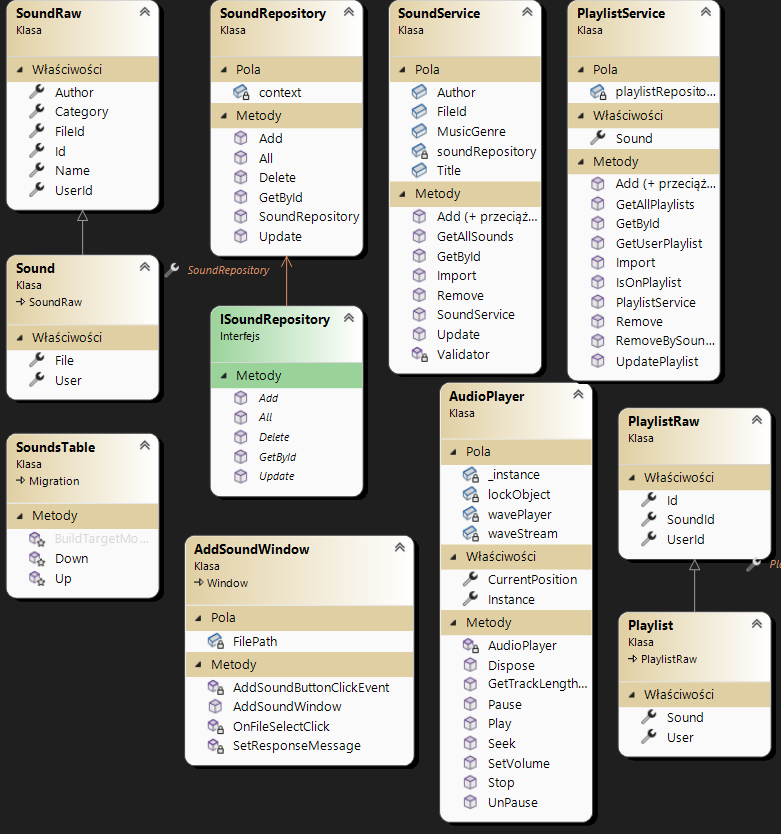
\includegraphics[width=500pt]{figures/diagram_cz1.png}
        \caption{{\footnotesize Diagram klas cześć 1}}
	\end{center}
\end{figure}


{Na przedstawionym diagramie widzimy tylko część klas projektu (jedną z czterech części całego diagramu). Rozmieszczenie tych klas nie jest bezpośrednio związane, gdyż obejmuje zarówno klasy repozytorium bazy danych, serwisy, pomocnicze klasy do migracji takie jak \texttt{SoundsTable}, jak i klasy tworzące interfejs użytkownika GUI, na przykład \texttt{AddSoundWindow}. Interesujące może być zastosowanie dziedziczenia klasy \texttt{SoundRaw} w klasie \texttt{Sound}. Rozwiązanie to jest stosowane tylko w wybranych przypadkach. Klasa \texttt{Sound} reprezentuje tabelę \texttt{Sounds}, o której będzie mowa później, ale definiuje również obiekty takie jak \texttt{File} oraz \texttt{User}, które są używane w relacjach między tabelami w bazie danych. Klasa \texttt{SoundRaw} definiuje wyłącznie kolumny w bazie (nie uwzględnia relacji), co jest potrzebne w kontekście importu i eksportu danych do formatu CSV.

Kolejnym interesującym aspektem jest zastosowanie wzorca Dependency Injection do wstrzykiwania klasy repozytorium \texttt{SoundRepository} w konstruktorze serwisu \texttt{SoundService}. Interfejs \texttt{ISoundRepository} definiuje metody, które nasze \texttt{SoundRepository} implementuje, a następnie instancja tego repozytorium jest wstrzykiwana do serwisu.



Klasa \texttt{SoundService} oferuje wszechstronne zarządzanie danymi, w tym operacje CRUD, walidację danych, import i eksport, a także obsługę błędów. Podobnie klasa \texttt{PlaylistService} umożliwia wykonanie tych samych operacji, jednak nie zajmuje się walidacją danych, gdyż nie operuje na danych wprowadzonych przez użytkownika, co sprawia, że jej obsługa jest nieco prostsza. Kolejnym kluczowym elementem przedstawionego diagramu jest klasa \texttt{AudioPlayer} – to ona przetwarza, odtwarza i zarządza dźwiękiem w aplikacji. Dysponuje metodami takimi jak \texttt{GetTrackLengthInSeconds()}, która zwraca długość aktualnie odtwarzanego utworu w sekundach, \texttt{SetVolume()} do regulacji głośności, a także \texttt{Play()}, \texttt{Stop()} i \texttt{Pause()} do kontrolowania odtwarzania utworu.
}

\begin{figure}[!ht]
	\begin{center}
	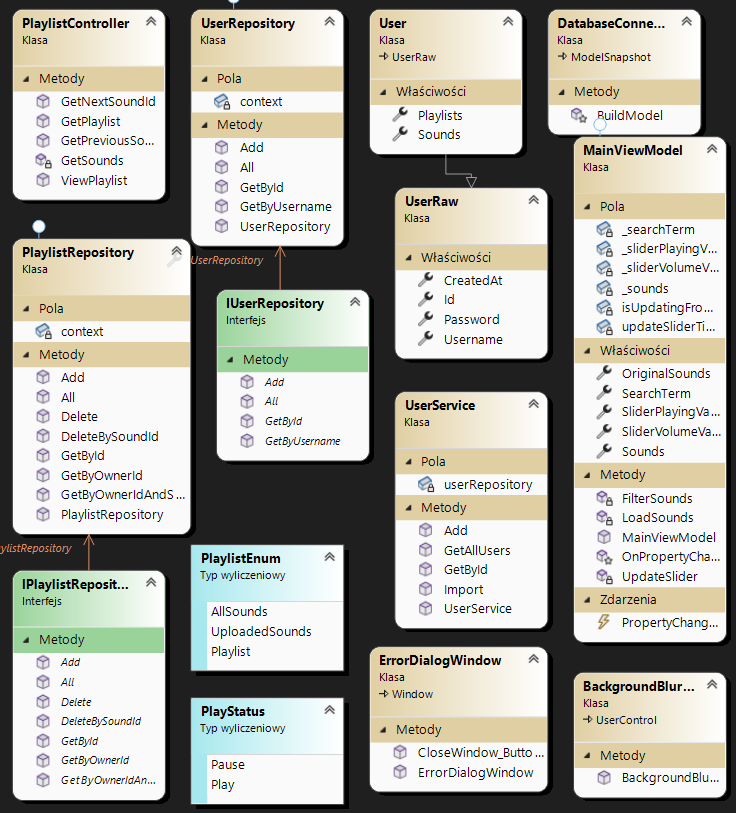
\includegraphics[width=500pt]{figures/diagram_czesc2.png}
        \caption{{\footnotesize Diagram klas cześć 2}}
	\end{center}
\end{figure}

\newpage

{Na kolejnym, drugim już diagramie, główną uwagę przykuwa klasa \texttt{MainViewModel}, która odpowiada za zarządzanie danymi między interfejsem użytkownika (UI) a logiką aplikacji. Odpowiada ona za odtwarzanie, wyszukiwanie, przewijanie, regulację głośności oraz kontrolowanie utworów. Opis reszty klas przedstawiono w punktach:}

\begin{enumerate}
    \item \textbf{ PlaylistController:} Klasa kontrolera zarządzająca playlistami. Posiada metody takie jak \newline \texttt{GetNextSoundId}, \texttt{GetPlaylist}, \texttt{GetPreviousSoundId}, \texttt{GetSounds}, \texttt{ViewPlaylist}, które służą do nawigacji i zarządzania listami odtwarzania w interfejsie użytkownika.
    \item \textbf{ UserRepository:} Repozytorium obsługujące operacje na danych użytkowników. Zawiera pola i metody niezbędne do realizacji operacji CRUD na użytkownikach, takie jak \texttt{Add}, \texttt{All}, \texttt{Delete}, \texttt{GetById}, \texttt{GetByUsername}.
    \item \textbf{ IUserRepository:}  Interfejs definiujący metody dostępu do danych użytkowników, których implementacja jest wymagana w \texttt{UserRepository}.
    \item \textbf{ User i UserRaw:} \texttt{User} definiuje tablice \texttt{Users} w bazie danych z relacją do tablic \texttt{Playlists} i \texttt{Sounds}. \texttt{UserRaw} reprezentuje surowe dane użytkownika, takie jak \texttt{Id}, \texttt{Password}, \texttt{Username}.
    \item \textbf{ UserService:} Serwis zapewniający logikę biznesową związaną z użytkownikami. Posiada pola i metody, takie jak \texttt{Add}, \texttt{GetAllUsers}, \texttt{GetById}, \texttt{Import}, które pozwalają na zarządzanie danymi użytkowników.
    \item \textbf{ DatabaseConnectionContextModelSnapshot:} Klasa \texttt{ModelSnapshot}, która zarządza wersjonowaniem modelu bazy danych..
    \item \textbf{ PlaylistRepository i IPlaylistRepository:}  Analogicznie do \texttt{UserRepository}, te klasy zarządzają operacjami na playlistach, z metodami do wykonania operacji CRUD.
    \item \textbf{ PlaylistEnum i PlayStatus:}  Typy wyliczeniowe, które definiują zbiór wartości, jakie mogą przyjąć playlisty (\texttt{AllSounds, UploadedSounds, Playlist}) oraz statusy odtwarzania (\texttt{Pause, Play}).
    \item \textbf{ ErrorDialogWindow:}  Klasa okna dialogowego służąca do wyświetlania komunikatów o błędach, posiada metodę taką jak \texttt{CloseWindow\_ButtonClick}.
    \item \textbf{ BackgroundBlur:}  Klasa \texttt{UserControl}, która służy do dodawania efektu rozmycia tła w interfejsie użytkownika.
\end{enumerate}

\begin{figure}[!ht]
	\begin{center}
	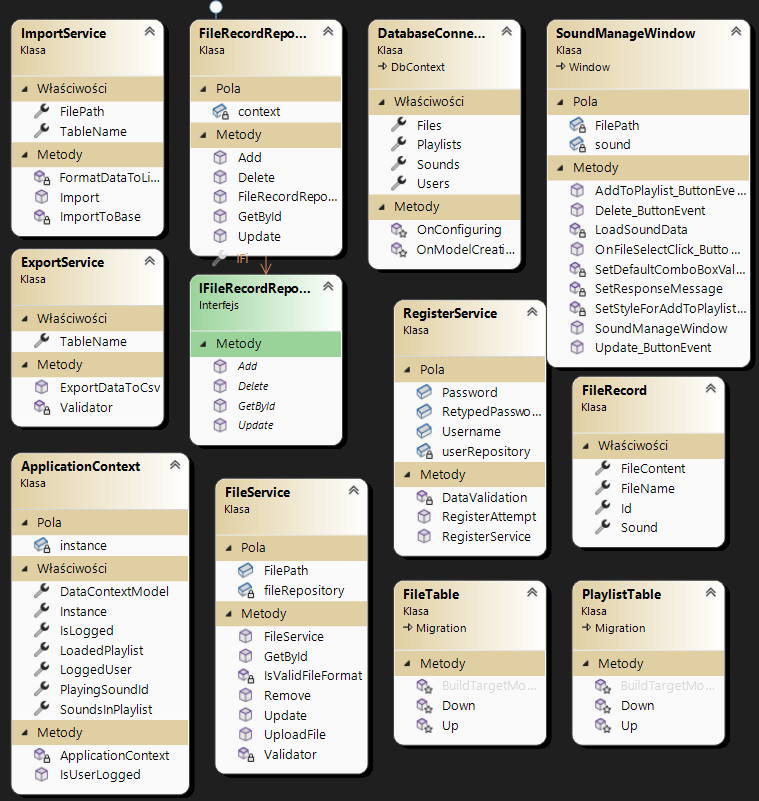
\includegraphics[width=500pt]{figures/diagram_czesc3.png}
        \caption{{\footnotesize Diagram klas cześć 3}}
	\end{center}
\end{figure}

\newpage
{Przedostatnia część diagramu, czyli trzecia, prezentuje nam klasę \texttt{ApplicationContext}. Klasa ta służy jako centralny punkt zarządzania stanem aplikacji i zawiera informacje o zalogowanym użytkowniku, załadowanej playliście i odtwarzanym dźwięku. Wykorzystuje ona wzorzec projektowy \texttt{Singleton}, który zapewnia stworzenie tylko jednej instancji klasy, co pozwala efektywnie przechowywać stan aplikacji. Opis reszty klas: }

\begin{enumerate}
    \item \textbf{ ImportService:} Klasa służąca do importowania danych. Posiada właściwości takie jak \texttt{FilePath} i \texttt{TableName}, a także metody \texttt{FormatDataToList}, \texttt{Import}, \texttt{ImportToBase}, które pozwalają na przetwarzanie i załadowanie danych do bazy danych.
    \item \textbf{ FileRecordRepository:} Repozytorium obsługujące operacje na rekordach plików. Zawiera standardowe metody CRUD: \texttt{Add}, \texttt{Delete}, \texttt{GetById}, \texttt{Update}.
    \item \textbf{ IFileRecordRepository:} Interfejs definiujący kontrakt dla \texttt{FileRecordRepository}, zapewniając oddzielenie implementacji od abstrakcji.
    \item \textbf{ ExportService:} Klasa odpowiedzialna za eksport danych. Posiada metody takie jak \newline \texttt{ExportDataToCsv} oraz \texttt{Validator}, które pozwalają na weryfikację i eksport danych do formatu CSV.
    \item \textbf{ DatabaseConnection:} Klasa z rozszerzeniem \texttt{DbContext}, używana przez Entity Framework do konfiguracji połączenia z bazą danych oraz definiowania modelu bazy danych za pomocą metod \texttt{OnConfiguring} i \texttt{OnModelCreating}.
    \item \textbf{ SoundManageWindow:} Klasa reprezentująca okno zarządzania dźwiękiem w interfejsie użytkownika. Zawiera metody do dodawania dźwięków do playlisty, usuwania, ładowania danych dźwiękowych, aktualizacji i innych interakcji z użytkownikiem.
    \item \textbf{ RegisterService:} Serwis obsługujący rejestrację użytkowników. Wykorzystuje \texttt{userRepository} do dostępu do danych użytkowników i zawiera metody \texttt{DataValidation}, \texttt{RegisterAttempt} do walidacji i próby rejestracji.
    \item \textbf{ FileService:} Serwis do zarządzania plikami, z metodami takimi jak \texttt{GetById}, \newline \texttt{IsValidFileFormat}, \texttt{Remove}, \texttt{Update}, \texttt{UploadFile}, \texttt{Validator}.
    \item \textbf{ FileRecord:} Klasa reprezentująca rekord pliku w tabeli \texttt{Files} w bazie danych MySQL z właściwościami takimi jak \texttt{FileContent}, \texttt{FileName}, \texttt{Id}, \texttt{Sound}.
    \item \textbf{ FileTable i PlaylistTable:} Klasy migracji, które są częścią Entity Framework Migrations i zawierają metody Up i Down do aktualizacji schematu bazy danych.
\end{enumerate}

\begin{figure}[!ht]
	\begin{center}
	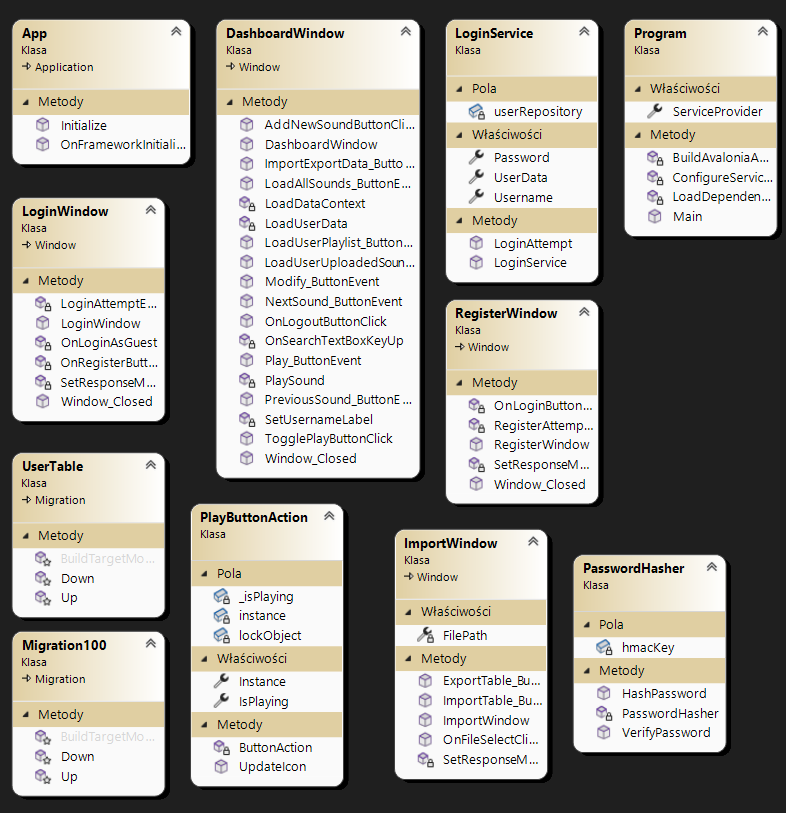
\includegraphics[width=500pt]{figures/diagram_czesc4.png}
        \caption{{\footnotesize Diagram klas cześć 3}}
	\end{center}
\end{figure}

\newpage

{Już ostatnia część diagramu prezentuje klasy takie jak \texttt{Program} (odpowiedzialna za uruchomienie aplikacji), \texttt{App} (inicjalizująca interfejs użytkownika w Avalonii) oraz \texttt{DashboardWindow}. \texttt{DashboardWindow} to klasa reprezentująca główne okno interfejsu użytkownika (Dashboard), przez które użytkownik może zarządzać aplikacją. Zawiera metody do zarządzania dźwiękiem, danymi oraz playlistami, takie jak \texttt{AddNewSoundButtonClickEvent}, \texttt{LoadData}, \texttt{LoadUserData}, \newline \texttt{TogglePlayButtonClick} i inne, co umożliwia interaktywną obsługę różnorodnych funkcji aplikacji. Opis pozostałych klas:}

\begin{enumerate}
    \item \textbf{ LoginService:} Serwis odpowiedzialny za proces logowania. Używa \texttt{userRepository} do dostępu do danych użytkownika i zawiera metody takie jak \texttt{LoginAttempt} do obsługi weryfikacji danych logowania.
    \item \textbf{ RegisterWindow:} Okno do rejestracji nowych użytkowników. Posiada metody takie jak \newline \texttt{OnLoginButtonClick}, \texttt{RegisterAttempt}, co pozwala na obsługę zdarzeń związanych z procesem rejestracji.
    \item \textbf{ UserTable i Migration100:} Klasy reprezentujące migracje bazy danych, używane do aktualizacji schematu bazy danych, z metodami \texttt{Up} i \texttt{Down}.
    \item \textbf{ PlayButtonAction:} Klasa, która zarządza stanem przycisku odtwarzania. Posiada pola określające stan odtwarzania \texttt{\_isPlaying} i metody takie jak \texttt{ButtonAction}, \texttt{UpdateIcon} co wskazuje na możliwość zmiany stanu przycisku odtwarzania.
    Dodatkowo, klasa ta jest tworzona jako pojedyncza instancja zgodnie z wzorcem projektowym Singleton.
    \item \textbf{ ImportWindow:} Okno do importowania danych do aplikacji. Zawiera metody \newline \texttt{ExportTableButtonClickEvent}, \texttt{OnFileSelectClick}, które pozwalają na interakcję z użytkownikiem podczas importowania danych z plików.
    \item \textbf{ PasswordHasher:} Klasa zawierająca metody do hashowania i weryfikacji haseł, takie jak \newline \texttt{HashPassword}, \texttt{VerifyPassword}, co jest istotne dla bezpieczeństwa danych użytkowników.
\end{enumerate}

\section{Zarządzenie danymi w aplikacji}

Schemat bazy danych MySQL wykorzystywanej przez aplikację:

\begin{figure}[!ht]
	\begin{center}
	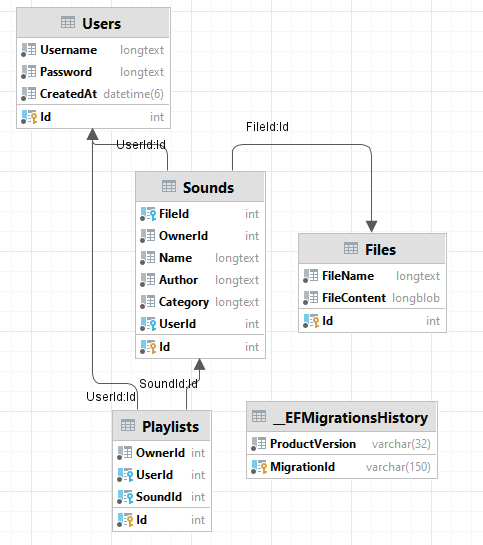
\includegraphics[height=300pt]{figures/schema.png}
        \caption{{\footnotesize Schema bazy danych}}
	\end{center}
\end{figure}

Na załączonym schemacie bazy danych aplikacji widoczne są cztery kluczowe tabele, które współgrają ze sobą, tworząc kompleksowy system zarządzania danymi:



\begin{enumerate}
    \item \textbf{Użytkownicy (Users):} Serce systemu stanowi tabela \texttt{Users}, przechowująca niezbędne informacje o użytkownikach, takie jak nazwa użytkownika (\texttt{Username}), hasło (\texttt{Password}) zahashowane przy pomocy algorytmu HMACSHA512, data utworzenia konta (\texttt{CreatedAt}) oraz unikalny identyfikator (\texttt{Id}). Ta tabela jest fundamentem dla autentykacji oraz zarządzania profilami użytkowników.
    \item \textbf{Dźwięki (Sounds):} Tabela \texttt{Sounds} służy jako repozytorium metadanych dla plików dźwiękowych w aplikacji. Każdy rekord dźwięku zawiera odniesienie do pliku (\texttt{FileId}), identyfikator właściciela (\texttt{OwnerId}), nazwę (\texttt{Name}), autora (\texttt{Author}), kategorię (\texttt{Category}) oraz unikalny identyfikator (\texttt{Id}). Powiązanie z tabelą \texttt{Users} za pomocą \texttt{UserId} umożliwia śledzenie, który użytkownik przesłał dany dźwięk, ułatwiając zarządzanie treścią i prawami własności.
    \item \textbf{Pliki (Files):} W tabeli \texttt{Files} przechowywane są właściwe dane plików dźwiękowych, takie jak zawartość pliku (\texttt{FileContent}) i nazwa pliku (\texttt{FileName}), każdy z unikalnym identyfikatorem (\texttt{Id}). Ta tabela działa jako magazyn danych binarnych, co pozwala na oddzielenie fizycznych plików od ich opisowych metadanych przechowywanych w tabeli Sounds.
    \item \textbf{Playlisty (Playlists):} Użytkownicy mogą tworzyć spersonalizowane playlisty za pośrednictwem tabeli \texttt{Playlists}, która zawiera odniesienia do ich twórców (\texttt{OwnerId}) oraz przypisane dźwięki (\texttt{SoundId}). Każda playlista posiada swój unikalny identyfikator (\texttt{Id}), co umożliwia łatwe odnajdywanie i zarządzanie kolekcjami dźwięków.
    \item \textbf{Historia Migracji EF (EFMigrationsHistory):} Specjalna tabela \texttt{\_EFMigrationsHistory} jest wykorzystywana przez Entity Framework do przechowywania historii migracji, które są niezbędne do aktualizacji i utrzymania integralności schematu bazy danych.

\end{enumerate}

Wszystkie te tabele łączą się w spójny system, który umożliwia dynamiczne zarządzanie danymi użytkowników, ich twórczością oraz preferencjami. Dzięki starannie przemyślanej architekturze i relacjom między tabelami, aplikacja jest w stanie zapewnić efektywne i bezproblemowe doświadczenia dla użytkownika, od logowania i rejestracji, przez przesyłanie i odtwarzanie dźwięków, aż po tworzenie i użytkowanie playlist.

Aplikacja umożliwia również import i eksport danych w formacie CSV, jednakże jest to ograniczone, ponieważ operacje te są problematyczne dla tabeli `Files`. Zawiera ona bardzo duże rekordy, które obejmują całe pliki piosenek. W związku z tym, w obecnej wersji aplikacji, import i eksport tabeli Files nie jest dostępny. Import innych tabel, takich jak `Users`, `Playlists` i `Sounds`, funkcjonuje natomiast bez zarzutu.



% ********** Koniec rozdziału **********
